\chapter{Grupos funcionales y familias}\label{ch:g11:functional-groups}

Abre una botella de vinagre, un frasco de quitaesmalte, una bolsa de
caramelos de pera, y pasa por delante de una pescadería: cuatro olores,
punzante, dulzón de \omterm{def:g6:solutions-and-solubility:solute}{disolvente}, afrutado y a pescado, y cuatro clases
distintas de \omterm{def:g7:atoms-and-molecules:molecule}{molécula}. Cada una debe su olor, y la mayor parte de su
química, no a su esqueleto carbonado, sino a un pequeño grupo de \omterm{def:g7:atoms-and-molecules:atom}{átomos}
unido a él: oxígeno e hidrógeno en un caso, un \omterm{def:g7:atoms-and-molecules:atom}{átomo} de nitrógeno en
otro. Los químicos clasifican los \omterm{def:g11:organic-skeletons:organic}{compuestos orgánicos} según esos
grupos.

\begin{recall}
Las \omterm{def:g11:organic-skeletons:formulas}{fórmulas esqueléticas}, los nombres de los \omterm{def:g11:organic-skeletons:alkane}{alcanos} y de los \omterm{def:g11:organic-skeletons:alkane}{grupos
alquilo}, los \omterm{def:g11:organic-skeletons:isomer}{isómeros} (\cref{ch:g11:organic-skeletons}). Los \omterm{def:g11:polarity-and-cohesion:polar-bond}{enlaces
polares} y los \omterm{def:g11:polarity-and-cohesion:hydrogen-bond}{enlaces de hidrógeno}
(\cref{ch:g11:polarity-and-cohesion}).
\end{recall}

\begin{omfigure}
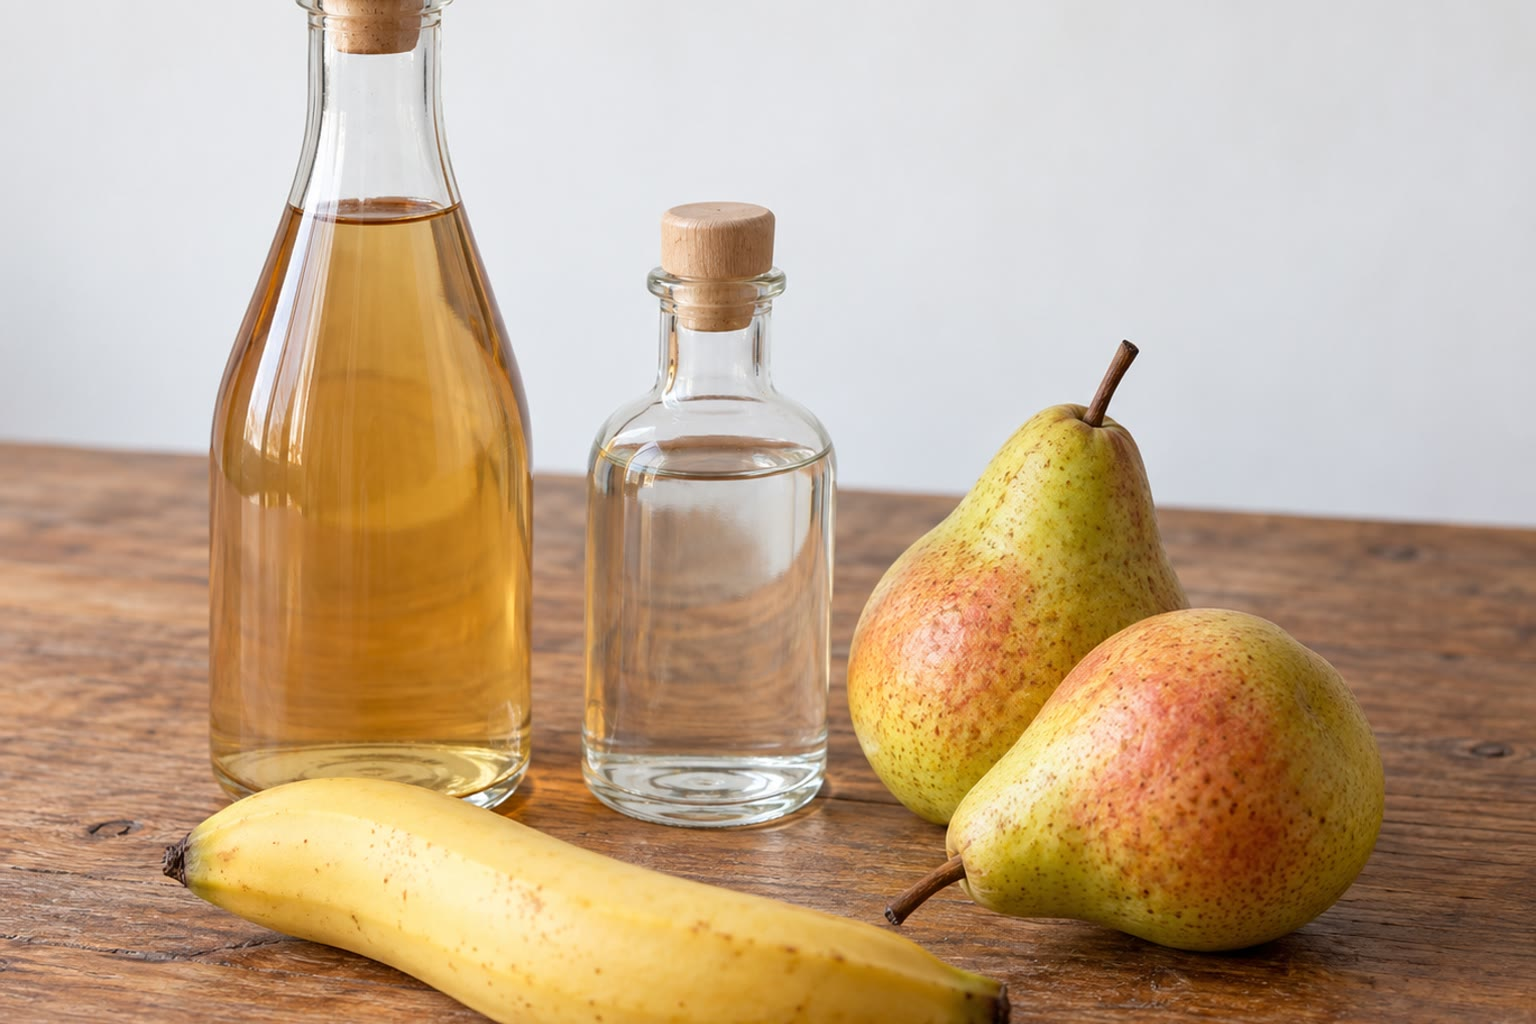
\includegraphics[width=0.5\linewidth]{images/book1/ai/g11-still-life-esters.jpg}

{\small Vinagre, un \omterm{def:g6:solutions-and-solubility:solute}{disolvente}, fruta: cada olor procede de un grupo de
\omterm{def:g7:atoms-and-molecules:atom}{átomos} distinto sobre un esqueleto carbonado.}
\end{omfigure}

\section{Los grupos funcionales}

\begin{definition}[Grupo funcional]\label{def:g11:functional-groups:functional-group}
Un \emph{grupo funcional}\index{grupo funcional} es un grupo de \omterm{def:g7:atoms-and-molecules:atom}{átomos},
distinto de los \omterm{def:g7:atoms-and-molecules:atom}{átomos} de carbono e hidrógeno del esqueleto unidos solo
por enlaces sencillos, que da a una \omterm{def:g7:atoms-and-molecules:molecule}{molécula} sus reacciones
características. Los compuestos que comparten un \omterm{def:g9:periodic-table-first-look:period}{grupo} funcional forman
una familia.
\end{definition}

\begin{omfigure}
\renewcommand{\arraystretch}{1.35}
\footnotesize
\begin{tabular}{@{}l@{\enspace}l@{\enspace}l@{\enspace}l@{\enspace}l@{}}
\hline
grupo & fórmula & familia & terminación & ejemplo \\
\hline
hidroxilo & \ce{-OH} & \omterm{def:g11:functional-groups:alcohol}{alcohol} & \emph{-ol} & etanol, \ce{CH3-CH2-OH} \\
carbonilo (extremo) & \ce{-CHO} & \omterm{def:g11:functional-groups:carbonyl}{aldehído} & \emph{-al} & etanal, \ce{CH3-CHO} \\
carbonilo (interior) & \ce{C-CO-C} & \omterm{def:g11:functional-groups:carbonyl}{cetona} & \emph{-ona} & propanona, \ce{CH3-CO-CH3} \\
carboxilo & \ce{-COOH} & \omterm{def:g11:functional-groups:carboxylic-acid}{ácido carboxílico} & ácido \emph{-oico} & ácido etanoico, \ce{CH3-COOH} \\
\omterm{def:g11:functional-groups:carboxylic-acid}{éster} & \ce{C-COO-C} & \omterm{def:g11:functional-groups:carboxylic-acid}{éster} & \emph{-ato de \ldots-ilo} & etanoato de etilo, \ce{CH3-COO-CH2-CH3} \\
\omterm{def:g11:functional-groups:amine}{amina} & \ce{-NH2} & \omterm{def:g11:functional-groups:amine}{amina} & \emph{-amina} & etanamina, \ce{CH3-CH2-NH2} \\
\omterm{def:g11:functional-groups:amine}{amida} & \ce{-CONH2} & \omterm{def:g11:functional-groups:amine}{amida} & \emph{-amida} & etanamida, \ce{CH3-CONH2} \\
\omterm{def:g10:electron-shells:family}{halógeno} & \ce{C-X} & \omterm{def:g11:functional-groups:halogenoalkane}{halogenoalcano} & prefijo \emph{cloro-}, \ldots & clorometano, \ce{CH3Cl} \\
\omterm{def:g10:lewis-and-shape:multiple-bond}{doble enlace} & \ce{C=C} & \omterm{def:g11:functional-groups:halogenoalkane}{alqueno} & \emph{-eno} & eteno, \ce{CH2=CH2} \\
\hline
\end{tabular}\par\medskip

\setchemfig{atom sep=1.4em}
\begin{tabular}{@{}c@{\quad}c@{\quad}c@{\quad}c@{\quad}c@{}}
\chemfig{R-C(=[2]O)-H} & \chemfig{R-C(=[2]O)-R'} & \chemfig{R-C(=[2]O)-O-H} &
\chemfig{R-C(=[2]O)-O-R'} & \chemfig{R-C(=[2]O)-N(-[1]H)-[7]H} \\
\small \omterm{def:g11:functional-groups:carbonyl}{aldehído} & \small \omterm{def:g11:functional-groups:carbonyl}{cetona} & \small \omterm{def:g11:functional-groups:carboxylic-acid}{ácido carboxílico} & \small \omterm{def:g11:functional-groups:carboxylic-acid}{éster} &
\small \omterm{def:g11:functional-groups:amine}{amida}
\end{tabular}\par\medskip

{\small Los principales \omterm{def:g11:functional-groups:functional-group}{grupos funcionales}, y los cinco construidos sobre
un grupo carbonilo \ce{C=O}, dibujados por completo. R y R$'$
representan cadenas carbonadas (\omterm{def:g11:organic-skeletons:alkane}{grupos alquilo}), y X, un \omterm{def:g7:atoms-and-molecules:atom}{átomo} de
\omterm{def:g10:electron-shells:family}{halógeno} (F, Cl, Br, I).}
\end{omfigure}

\section{Los alcoholes y su clase}

\begin{definition}[Alcohol, clase de un alcohol]\label{def:g11:functional-groups:alcohol}
Un \emph{alcohol}\index{alcohol} tiene un grupo hidroxilo \ce{-OH} unido
a un \omterm{def:g7:atoms-and-molecules:atom}{átomo} de carbono que solo tiene enlaces sencillos. La \emph{clase
de un alcohol}\index{clase de un alcohol} es primaria, secundaria o
terciaria según que el \omterm{def:g7:atoms-and-molecules:atom}{átomo} de carbono que lleva el \ce{-OH} esté unido
a uno, dos o tres \omterm{def:g7:atoms-and-molecules:atom}{átomos} de carbono más. (El metanol, \ce{CH3OH}, cuyo
carbono no está unido a ninguno, se cuenta entre los alcoholes
primarios.)
\end{definition}

\begin{omfigure}
\setchemfig{atom sep=1.9em}
\begin{tabular}{ccc}
\chemfig{-[:30]-[:-30]-[:30]-[:-30]OH} &
\chemfig{-[:30](-[:90]OH)-[:-30]-[:30]} &
\chemfig{-[:0](-[:90]OH)(-[:-90])-[:0]} \\[4pt]
\small butan-1-ol & \small butan-2-ol & \small 2-metilpropan-2-ol \\
\small \textbf{primario} & \small \textbf{secundario} & \small \textbf{terciario} \\
\small (C del \ce{-OH}: 1 carbono vecino) & \small (2 vecinos) &
\small (3 vecinos)
\end{tabular}

{\small Tres \omterm{def:g11:organic-skeletons:isomer}{isómeros} \ce{C4H10O}, tres clases de \omterm{def:g11:functional-groups:alcohol}{alcohol}.}
\end{omfigure}

\section{Aldehídos, cetonas, ácidos y ésteres}

\begin{definition}[Aldehído, cetona]\label{def:g11:functional-groups:carbonyl}
Un grupo carbonilo es un \omterm{def:g10:lewis-and-shape:multiple-bond}{doble enlace} \ce{C=O}. Si su \omterm{def:g7:atoms-and-molecules:atom}{átomo} de carbono
está en el extremo de la cadena (unido al menos a un \omterm{def:g7:atoms-and-molecules:atom}{átomo} de
hidrógeno), el compuesto es un \emph{aldehído}\index{aldehido@aldehído}; si está
en el interior de la cadena (unido a dos \omterm{def:g7:atoms-and-molecules:atom}{átomos} de carbono), el
compuesto es una \emph{cetona}\index{cetona}.
\end{definition}

\begin{definition}[Ácido carboxílico, éster]\label{def:g11:functional-groups:carboxylic-acid}
Un \emph{ácido carboxílico}\index{acido carboxilico@ácido carboxílico} tiene un grupo
carboxilo \ce{-COOH}, un carbonilo y un hidroxilo sobre el mismo \omterm{def:g7:atoms-and-molecules:atom}{átomo}
de carbono. Un \emph{éster}\index{ester@éster} tiene el grupo \ce{-COO-} entre
dos cadenas carbonadas: está relacionado con un ácido cuyo \ce{-OH} se
ha sustituido por un \ce{-O-}R$'$ procedente de un \omterm{def:g11:functional-groups:alcohol}{alcohol}.
\end{definition}

\begin{example}[El etanoato de etilo]\label{ex:g11:functional-groups:ethyl-ethanoate}
El \omterm{def:g6:solutions-and-solubility:solute}{disolvente} etanoato de etilo, \ce{CH3-COO-CH2-CH3}, huele a
caramelos de pera y a quitaesmalte. Su ``parte ácida'', \ce{CH3-CO},
procede del ácido etanoico \ce{CH3-COOH} y da la primera palabra del
nombre, \emph{etanoato}; su ``parte alcohólica'', \ce{O-CH2-CH3}, procede
del etanol \ce{CH3-CH2-OH} y da el final, \emph{de etilo}. Un capítulo
posterior muestra cómo se fabrica un \omterm{def:g11:functional-groups:carboxylic-acid}{éster} a partir de su ácido y de su
\omterm{def:g11:functional-groups:alcohol}{alcohol}.
\end{example}

\begin{omfigure}
\setchemfig{atom sep=2.2em}
\chemfig{@{a}H_3C-@{c}C(=[2]@{o}O)-@{x}O-CH_2-@{z}CH_3}
\chemmove{
  \fill[omProp, opacity=0.14, rounded corners]
    ($(a.south west)+(-0.12,-0.15)$) rectangle ($(o.north east)+(0.25,0.12)$);
  \fill[omDef, opacity=0.14, rounded corners]
    ($(x.south west)+(-0.2,-0.15)$) rectangle ($(z.north east)+(0.4,0.75)$);
  \node[omProp, anchor=north east, align=right, font=\small] at ($(c.south)+(0.15,-0.25)$)
    {parte ácida, del ácido etanoico:\\ \emph{etanoato}};
  \node[omDef, anchor=north west, align=left, font=\small] at ($(x.south)+(0.05,-0.25)$)
    {parte alcohólica, del etanol:\\ \emph{de etilo}};}
\par\vspace{1.4cm}

{\small Nombrar un \omterm{def:g11:functional-groups:carboxylic-acid}{éster}: la parte ácida da un nombre terminado en
\emph{-ato} (\emph{etanoato}), y la parte alcohólica, un nombre de
alquilo (\emph{etilo}) introducido por ``de''; el nombre es
``etanoato de etilo''.}
\end{omfigure}

\section{Aminas, amidas, halogenoalcanos y alquenos}


\begin{definition}[Amina, amida]\label{def:g11:functional-groups:amine}
Una \emph{amina}\index{amina} tiene un \omterm{def:g7:atoms-and-molecules:atom}{átomo} de nitrógeno unido a una
cadena carbonada por un enlace sencillo, como en \ce{-NH2}. Una
\emph{amida}\index{amida} tiene un \omterm{def:g7:atoms-and-molecules:atom}{átomo} de nitrógeno unido al carbono
de un grupo carbonilo, como en \ce{-CO-NH2}.
\end{definition}

\begin{definition}[Halogenoalcano, alqueno]\label{def:g11:functional-groups:halogenoalkane}
Un \emph{halogenoalcano}\index{halogenoalcano} es un \omterm{def:g11:organic-skeletons:alkane}{alcano} en el que
uno o varios \omterm{def:g7:atoms-and-molecules:atom}{átomos} de hidrógeno se han sustituido por \omterm{def:g7:atoms-and-molecules:atom}{átomos} de
\omterm{def:g10:electron-shells:family}{halógeno} (F, Cl, Br, I). Un \emph{alqueno}\index{alqueno} tiene un \omterm{def:g10:lewis-and-shape:multiple-bond}{doble
enlace} carbono--carbono, \ce{C=C}.
\end{definition}

\begin{remark}[Olores y grupos]\label{rem:g11:functional-groups:smells}
Muchas \omterm{def:g11:functional-groups:amine}{aminas} pequeñas huelen a pescado podrido, y el olor del pescado
que ya no está fresco se debe en gran parte a ellas. Muchos \omterm{def:g11:functional-groups:carboxylic-acid}{ésteres}
pequeños huelen a fruta. Los \omterm{def:g11:functional-groups:carboxylic-acid}{ácidos carboxílicos} pequeños tienen un olor
punzante, como el vinagre; la propanona, una \omterm{def:g11:functional-groups:carbonyl}{cetona}, es el olor familiar
a \omterm{def:g6:solutions-and-solubility:solute}{disolvente} del quitaesmalte.
\end{remark}

\section{Nombrar}

\begin{method}[Nombrar un compuesto orgánico con un grupo funcional]\label{met:g11:functional-groups:naming}
\begin{enumerate}
  \item Buscar la cadena carbonada más larga que \emph{contiene} el
        carbono del \omterm{def:g11:functional-groups:functional-group}{grupo funcional} (o, para un \omterm{def:g11:functional-groups:alcohol}{alcohol} o una \omterm{def:g11:functional-groups:amine}{amina}, el
        carbono que lo lleva): da la raíz.
  \item Numerar la cadena desde el extremo que da al \omterm{def:g11:functional-groups:functional-group}{grupo funcional} el
        número más bajo.
  \item Sustituir la \emph{-o} final del \omterm{def:g11:organic-skeletons:alkane}{alcano} por la terminación de la
        familia, precedida si hace falta de la posición del grupo:
        propan-2-ol, butan-2-ona. (Los \omterm{def:g11:functional-groups:carbonyl}{aldehídos}, los ácidos y las
        \omterm{def:g11:functional-groups:amine}{amidas} tienen su grupo en el carbono 1: sin número.)
  \item Añadir los sustituyentes alquilo como prefijos, con sus
        posiciones, como en los \omterm{def:g11:organic-skeletons:alkane}{alcanos}; un \omterm{def:g10:electron-shells:family}{halógeno} es siempre un
        prefijo (2-cloropropano).
\end{enumerate}
\end{method}

\begin{example}[Cuatro nombres]\label{ex:g11:functional-groups:names}
\setchemfig{atom sep=1.7em}
\chemfig{-[:30](-[:90]OH)-[:-30]} es el propan-2-ol (un \omterm{def:g11:functional-groups:alcohol}{alcohol}
secundario);
\chemfig{-[:30](=[:90]O)-[:-30]-[:30]} es la butan-2-ona;
\chemfig{-[:30]-[:-30]-[:30](=[:90]O)-[:-30]OH} es el ácido butanoico;
\chemfig{-[:30](-[:90])-[:-30]-[:30]=[:-30]O} es el 3-metilbutanal.
\end{example}

\begin{omfigure}
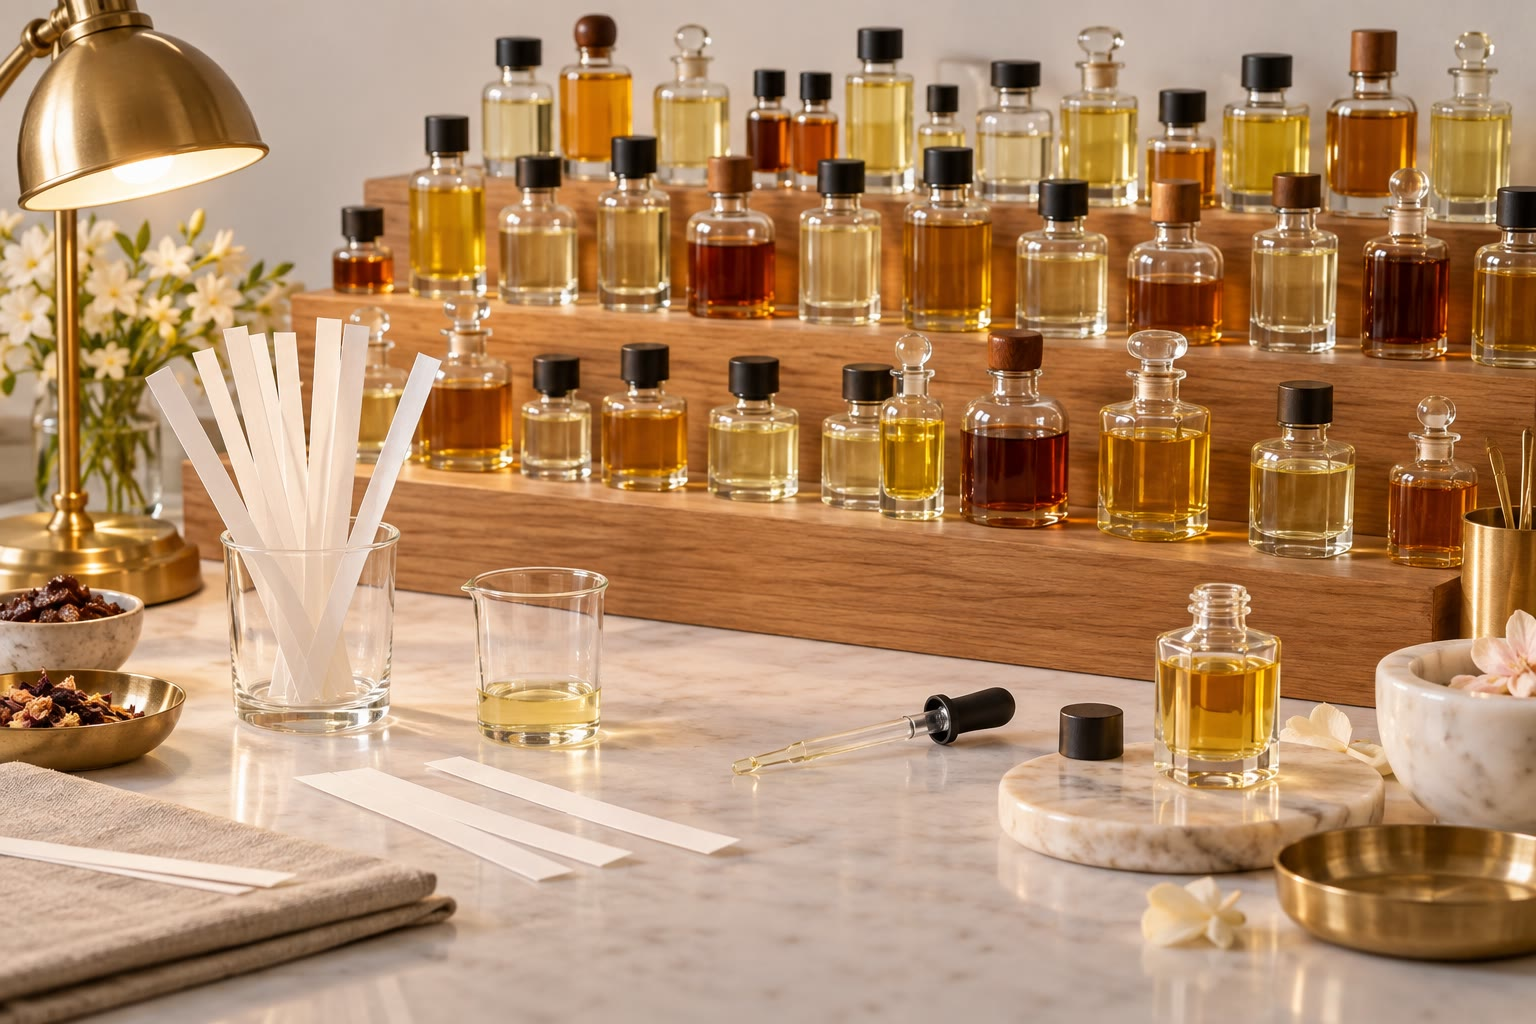
\includegraphics[width=0.48\linewidth]{images/book1/ai/g11-perfumer-lab.jpg}

{\small La mesa de trabajo de un perfumista: muchos frascos contienen
\omterm{def:g11:functional-groups:carboxylic-acid}{ésteres}, \omterm{def:g11:functional-groups:alcohol}{alcoholes}, \omterm{def:g11:functional-groups:carbonyl}{aldehídos} y \omterm{def:g11:functional-groups:carbonyl}{cetonas}.}
\end{omfigure}

\begin{safety}{\ghs[0.82cm]{GHS02}\ghs[0.82cm]{GHS05}\ghs[0.82cm]{GHS07}}
% ledger: ghs:acetone, ghs:acetic-acid
La propanona es muy inflamable e irrita los ojos; sus vapores provocan
somnolencia. El ácido etanoico puro es inflamable y provoca quemaduras
graves en la piel y en los ojos; el vinagre es una disolución diluida de
él. Los olores nunca se prueban oliendo directamente un matraz: el vapor
se acerca suavemente a la nariz con la mano, y solo cuando lo dice el
profesor.
\end{safety}

\section{Ejercicios}


\begin{exercise}[$\star$]\label{exo:g11:functional-groups:1}
Nombra el \omterm{def:g11:functional-groups:functional-group}{grupo funcional} y la familia de cada compuesto:
\ce{CH3-CH2-CH2-OH}; \ce{CH3-CO-CH2-CH3}; \ce{CH3-CH2-COOH};
\ce{CH3-COO-CH3}; \ce{CH3-CH2-NH2}.
\end{exercise}

\begin{exercise}[$\star$]\label{exo:g11:functional-groups:2}
Nombra: \ce{CH3-OH}; \ce{CH3-CH2-CH2-OH}; \ce{HCOOH}; \ce{CH3-CH2-CHO};
\ce{CH3-CO-CH3}.
\end{exercise}

\begin{exercise}[$\star$]\label{exo:g11:functional-groups:3}
¿A qué familia pertenece cada compuesto: butan-2-ol, pentanal,
propanoato de metilo, propanamida, 2-bromopropano, but-1-eno?
\end{exercise}

\begin{exercise}[$\star$]\label{exo:g11:functional-groups:4}
Escribe las \omterm{def:g11:organic-skeletons:formulas}{fórmulas semidesarrolladas} del propanal y de la propanona.
¿Cuál es el \omterm{def:g11:functional-groups:carbonyl}{aldehído}? ¿Cómo lo sabes?
\end{exercise}

\begin{exercise}[$\star$]\label{exo:g11:functional-groups:5}
Da la clase del propan-1-ol, del propan-2-ol y del 2-metilpropan-2-ol.
\end{exercise}

\begin{exercise}[$\star\star$]\label{exo:g11:functional-groups:6}
Dibuja las \omterm{def:g11:organic-skeletons:formulas}{fórmulas esqueléticas} del pentan-3-ol, el ácido
2-metilbutanoico, la hexan-2-ona y el etanoato de propilo.
\end{exercise}

\begin{exercise}[$\star\star$]\label{exo:g11:functional-groups:7}
El propanal y la propanona tienen la misma \omterm{def:g11:organic-skeletons:formulas}{fórmula molecular}. Dala. ¿Son
\omterm{def:g11:organic-skeletons:isomer}{isómeros}? ¿Tienen el mismo \omterm{def:g11:functional-groups:functional-group}{grupo funcional}?
\end{exercise}

\begin{exercise}[$\star\star$]\label{exo:g11:functional-groups:8}
Escribe la \omterm{def:g11:organic-skeletons:formulas}{fórmula semidesarrollada} y el nombre del \omterm{def:g11:functional-groups:carboxylic-acid}{éster} cuya parte
ácida procede del ácido metanoico \ce{HCOOH} y cuya parte alcohólica
procede del etanol; después, los del \omterm{def:g11:functional-groups:carboxylic-acid}{éster} del ácido etanoico y el
propan-1-ol.
\end{exercise}

\begin{exercise}[$\star\star$]\label{exo:g11:functional-groups:9}
Nombra los \omterm{def:g11:functional-groups:carboxylic-acid}{ésteres} \ce{CH3-COO-CH3}, \ce{CH3-CH2-COO-CH2-CH3} y
\ce{HCOO-CH3}, y da el ácido y el \omterm{def:g11:functional-groups:alcohol}{alcohol} con los que está relacionado
cada uno.
\end{exercise}

\begin{exercise}[$\star\star$]\label{exo:g11:functional-groups:10}
Dibuja y nombra los cuatro \omterm{def:g11:functional-groups:alcohol}{alcoholes} de fórmula \ce{C4H10O}, y da la
clase de cada uno.
\end{exercise}

\begin{exercise}[$\star\star$]\label{exo:g11:functional-groups:11}
Con la tabla de grupos: ¿cuál es la familia de \ce{CH3-CO-NH2}? ¿Qué
terminación lleva el nombre de un \omterm{def:g11:functional-groups:halogenoalkane}{alqueno}? ¿Qué familias tienen un
grupo carbonilo con un \omterm{def:g7:atoms-and-molecules:atom}{átomo} de oxígeno o de nitrógeno sobre el mismo
carbono?
\end{exercise}

\begin{exercise}[$\star\star\star$]\label{exo:g11:functional-groups:12}
Rodea con un círculo y nombra los \omterm{def:g11:functional-groups:functional-group}{grupos funcionales} de la aspirina y del
paracetamol. (Un \ce{-OH} unido directamente a un anillo como el del
paracetamol se llama grupo fenol; se comporta de forma distinta a un
\omterm{def:g11:functional-groups:alcohol}{alcohol}.)
\begin{center}
\setchemfig{atom sep=1.6em}
\chemfig{*6(-=-(-COOH)=(-O-[:150]C(=[:90]O)-[:210]H_3C)-=)}
\qquad
\chemfig{*6((-OH)=-=(-N(-[2]H)-[7]C(=[6]O)-[1]CH_3)-=-)}
\\[2pt] \small aspirina \hspace{4.2cm} paracetamol
\end{center}
\end{exercise}

\begin{exercise}[$\star\star\star$]\label{exo:g11:functional-groups:13}
% ledger: bp:C2H5OH, bp:CH3OCH3
El etanol \ce{CH3-CH2-OH} y el metoximetano \ce{CH3-O-CH3} tienen la
misma \omterm{def:g11:organic-skeletons:formulas}{fórmula molecular}. Dala. El metoximetano pertenece a una familia
que no está en la tabla, los éteres. ¿Cuál de los dos puede formar
\omterm{def:g11:polarity-and-cohesion:hydrogen-bond}{enlaces de hidrógeno} entre sus propias \omterm{def:g7:atoms-and-molecules:molecule}{moléculas}? ¿Cuál hierve a mayor
temperatura (uno hierve a \qty{78}{\celsius}, y el otro, a
\qty{-25}{\celsius})?
\end{exercise}

\begin{exercise}[$\star\star\star$]\label{exo:g11:functional-groups:14}
El ácido láctico, que producen los músculos cansados, es
\chemfig{CH_3-CH(-[2]OH)-COOH}. Nombra sus dos \omterm{def:g11:functional-groups:functional-group}{grupos funcionales}.
Cuando una \omterm{def:g7:atoms-and-molecules:molecule}{molécula} tiene un grupo ácido y otro grupo, el ácido da la
terminación y el otro grupo pasa a ser un prefijo (\emph{hidroxi-} para
\ce{-OH}, \emph{amino-} para \ce{-NH2}). Nombra el ácido láctico y,
después, la glicina, \ce{H2N-CH2-COOH}.
\end{exercise}

\begin{exercise}[$\star\star\star$]\label{exo:g11:functional-groups:15}
El vino que se deja al \omterm{def:g4:air-a-mixture-of-gases:air}{aire} se convierte en vinagre: el etanol pasa a
ácido etanoico, a través del etanal. Escribe las \omterm{def:g11:organic-skeletons:formulas}{fórmulas
semidesarrolladas} y moleculares de los tres compuestos y sus familias.
¿Qué cambia en la fórmula en cada paso?
\end{exercise}

\section{Problema: Aromas de fruta}

\begin{problem}[{Problema de fin de semana --- una química de aromas
construye el olor del plátano: ¿cuál es la masa molar de la molécula
clave?}]
\label{pb:g11:functional-groups:1}
% ledger: aw:C, aw:H, aw:O
Una química de aromas tiene cinco compuestos sobre su mesa:
\begin{center}
\begin{tabular}{ll}
A & \chemfig{CH_3-C(=[2]O)-O-CH_2-CH_2-CH(-[2]CH_3)-CH_3} \\[16pt]
B & \chemfig{HO-CH_2-CH_2-CH(-[2]CH_3)-CH_3} \\[10pt]
C & \ce{CH3-COOH} \\
D & \ce{CH3-CH2-CH2-CH2-CH2-CHO} \\
E & \ce{CH3-CH2-CH2-COO-CH2-CH3}
\end{tabular}
\end{center}
A huele a plátano y a caramelos de pera; B, a malta; C, a vinagre; D, a
hierba recién cortada; E, a piña.

\medskip
\noindent\textbf{Parte I --- Grupos y familias.}
\begin{enumerate}
  \item Nombra el \omterm{def:g11:functional-groups:functional-group}{grupo funcional} de cada compuesto.
  \item Da la familia de cada uno.
  \item ¿Qué compuestos son \omterm{def:g11:functional-groups:carboxylic-acid}{ésteres}? ¿Qué olores tienen?
  \item ¿Cuál es la clase del \omterm{def:g11:functional-groups:alcohol}{alcohol} B?
  \item Da la \omterm{def:g11:organic-skeletons:formulas}{fórmula molecular} de D, y dibuja un \omterm{def:g11:organic-skeletons:isomer}{isómero} de D que sea
        una \omterm{def:g11:functional-groups:carbonyl}{cetona}.
\end{enumerate}

\medskip
\noindent\textbf{Parte II --- Nombres.}
\begin{enumerate}[resume]
  \item Nombra B (busca la cadena más larga que contiene el carbono que
        lleva el \ce{-OH}).
  \item Nombra C y D.
  \item Nombra E, y da el ácido y el \omterm{def:g11:functional-groups:alcohol}{alcohol} con los que está
        relacionado.
  \item Explica el nombre de A, etanoato de 3-metilbutilo: ¿qué parte
        procede del ácido y cuál del \omterm{def:g11:functional-groups:alcohol}{alcohol}?
\end{enumerate}

\medskip
\noindent\textbf{Parte III --- A partir de un ácido y un \omterm{def:g11:functional-groups:alcohol}{alcohol}.}
\begin{enumerate}[resume]
  \item ¿Con qué dos compuestos de la mesa está relacionado A?
  \item Da las \omterm{def:g11:organic-skeletons:formulas}{fórmulas moleculares} de A, B y C.
  \item Un \omterm{def:g11:functional-groups:carboxylic-acid}{éster} se fabrica a partir de su ácido y de su \omterm{def:g11:functional-groups:alcohol}{alcohol} con
        pérdida de una \omterm{def:g7:atoms-and-molecules:molecule}{molécula} pequeña. Con las fórmulas, averigua
        cuál.
  \item Escribe la ecuación de la formación de A, con \omterm{def:g11:organic-skeletons:formulas}{fórmulas
        moleculares}, y comprueba que está ajustada.
\end{enumerate}

\medskip
\noindent\textbf{Parte IV --- \omterm{def:g10:the-mole:molar-mass}{Masas molares}.}
\begin{enumerate}[resume]
  \item Calcula las \omterm{def:g10:the-mole:molar-mass}{masas molares} de B y de C.
  \item Deduce la \omterm{def:g10:the-mole:molar-mass}{masa molar} de A a partir de la ecuación de la
        pregunta 13.
  \item Calcula la \omterm{def:g10:the-mole:molar-mass}{masa molar} de A directamente a partir de su fórmula,
        y compáralas.
  \item Se halla que una muestra afrutada desconocida tiene una \omterm{def:g10:the-mole:molar-mass}{masa
        molar} cercana a \qty{116}{g/mol}. ¿Es A o E?
  \item El ácido heptanoico, \ce{CH3-(CH2)5-COOH}, huele a rancio.
        Muestra que es un \omterm{def:g11:organic-skeletons:isomer}{isómero} de A. ¿Puede una \omterm{def:g10:the-mole:molar-mass}{masa molar}, por sí
        sola, identificar un compuesto?
  \item ¿Por qué dicen los químicos que el olor pertenece tanto al \omterm{def:g11:functional-groups:functional-group}{grupo
        funcional} como al esqueleto? Usa A y el ácido heptanoico.
  \item Da la respuesta final: ¿cuál es la \omterm{def:g10:the-mole:molar-mass}{masa molar} del \omterm{def:g11:functional-groups:carboxylic-acid}{éster} del
        plátano, el etanoato de 3-metilbutilo?
\end{enumerate}
\end{problem}
